\documentclass{article}
\usepackage[utf8]{inputenc}
\usepackage{amsmath}
\usepackage{amsfonts}
\usepackage{graphicx}

\begin{document}

\title{Solution to Mock contest.}
\author{Prajit Adhikari}
\maketitle

\begin{enumerate}
\item Let $a_0,a_1,...,a_n$ be real numbers satisfying $a_0 = a_n = 0$ and $$a_{i+1} -2a_{i} + a_{i-1} = a_{i}^2$$ for $i = 1,2,...,n -1$. Prove that $a_i \leq 0$ for $i = 1,2,..., n-1$.\\
    \textbf{Solution:}\\
    Adding the expression for $i=1,2,....n-1$, we get,
    $$ a_1^2+a_2^2+........+a_{n-1}^2 = -(a_1+a_{n-1}) $$
    Similarly,$a_{i+1}+a_{i-1}+1=(a_i+1)^2.....(i)$.\\
    We know, $a_1+a_{n-1} \leq 0$. By equation $(i)$ it is clear that for $a_i=0$ for $i=1,....N-1$, then all $a_i$'s are zero. So, we only deal with cases when $a_i$'s are less than zero.\\
    Case I: $a_1 < 0$, then
    $$a_2+1= (a_1+1)^2 \implies a_2 <0 since, (a_1+1)^2<1$$
    This implies that all $a_i$'s are less than 0.
    Case II: $a_{n-1}<0$, then,
    $$ a_{n-1}+1 = (a_{n-2}+1)^2$$
    Since, $a_{n-1}+1 < 1 \implies a_{n-2}<1$. \\
    Using similar arguments in both cases and  we get that $a_i\leq 0$ for $i=1,2,.........,n-1$. QED
    
    \newpage
    
    \item  Suppose that for a prime number p and integers a,b,c the following holds: $$6 | p + 1, p | a + b + c, p | a^4 + b^4 + c^4$$. Prove that $p | a,b,c$.\\
    \textbf{Solution:}\\
    We have that,
    $$a^4+b^4+c^4 = ((a+b+c)^2-2ab-2bc-2ca)^2-2a^2b^2-2b^2c^2-2c^2a^2$$
    Since, $p|a+b+c, p=6k-1$, we have that,
    $$p|(2ab+2bc+2ca)^2-2a^2b^2-2b^2c^2-2c^2a^2$$
    Let, $ab=x,bc=y$ and $ca=z$. Then,
    $$p|2(x+y+z)^2-x^2-y^2-z^2\implies p|x^2+y^2+z^2+4xy+4yz+4zx$$
    Now,
    $$ p|a^2b^2+b^2c^2+c^2a^2+4ab^2c+4a^2bc+4abc^2$$
    $$p|a^2b^2+b^2c^2+c^2a^2+4abc(a+b+c) \implies p|x^2+y^2+z^2$$
    Then,
    $$p|a^4+b^4+c^4+2(a^2b^2+b^2c^2+c^2a^2) \implies 2|(a^2+b^2+c^2)^2$$
    $$\implies p|a^2+b^2+c^2 \implies p|ab+bc+ac \implies p|b(a+c)+ac$$
    Now,
    $$p|b(a+c)+ac-b(a+b+c) \implies p|ac-b^2, p|bc-a^2$$
    $$p|a^2+b^2+c^2+ac-b^2+bc-a^2 \implies p|c^2+ac+bc \implies p|c(a+b+c)$$
    Hence, $$p|c \implies p|bc-a^2 \implies p|a \implies p|b$$.
    Therefore, $p|a,b,c$. QED
    
\newpage
    
  \item  Let $a$ be any integer. Define the sequence $x_0,x_1,...$ by 
  $x_0 = a, x_1 = 3$, and for all $n > 1$,
    $$x_n = 2x_{n-1} -4x_{n-2} + 3$$.
    Determine the largest integer $k_a$ for which there exists a prime $p$ such that $p^{k_a}$ divides $x_{2011} -1$.\\
    \textbf{Solution:}\\
    Let, $y_n=x_n-1$ be a sequence. Then,
    $$y_n=2y_{n-1}-4y_{n-2}$$
    Using above identity, we get,
    $$y_n=2(2y_{n-2}-4y_{n-3})-4y_{n-2} \implies y_n=-8y_{n-3}$$
    Since $n$ was arbitrarily chosen, we have that for any $\{n,n-1,n-2\}$ divisible by three, the above statement must apply. So, for $m$ divisible by 3, we get,\\
     $y_m = (-1)^m 2^m y_0 \implies 2^m | y^m$. Hence, for $m=2011$, we have that greatest $k_a$ which divides $a_{2011}-1$ is $\boxed{2011}$.
    
    
    \newpage
    
    \item  (a) Show that the equation $\lfloor x \rfloor (x^2 + 1) = x^3$, where $\lfloor x \rfloor$ denotes the largest integer not larger than x, has exactly one real solution in each interval between consecutive positive integers. \\
    (b) Show that none of the positive real solutions of this equation is rational. \\
    \textbf{Solution:}\\
   (a). Let, $\lfloor x \rfloor =x +\{x\}$, where $\{x\}$ is the fractional part of the number. Suppose, $\{x\}=m$ and $\lfloor x \rfloor =k$.\\
    Then, $x=m+k$, now, $(x-\{x\})(x^2+1)=x^3 \implies x=m(x^2+1) \implies m+k =m(m+k)^2+m\implies k=m(m+k)^2$. \\
    For an interval $(k,k+1)$, we see that the above function in $m$ is monotonous for increasing positive interval. Hence, for $k \to k+1$, we have that $(m+1)(m+k+1)^2>k$ whereas $m(m+k)<k$, since $m<1$ and $m \not =0$. Finally, we see by mean value theorem that there exists a $m$ for every interval $(k,k+1)$, so there is exactly one solution as the function is also increasing monotonously.\\
    
    (b). Let, $x=\frac{p}{q}$ such that $gcd(p,q)=1$. then we have,
    $$kq(p^2+q^2)=p^3$$
    Since, $k,p,q \in \mathbb{Z}$, we have,
    $q|p^3 \implies gcd(p,q)\not = 1$, which is absurd. So, there is no rational solution. QED.
    
    
    
    
    
    \newpage
    
    \item Let O be the circumcenter of the triangle ABC. The segment XY is the diameter of the circumcircle perpendicular to BC and it meets BC at M. The point X is closer to M than Y and Z is the point on MY such that MZ = MX. The point W is the midpoint of AZ. a) Show that W lies on the circle through the midpoints of the sides of ABC; b) Show that MW is perpendicular to AY.\\
    \textbf{Solution:}\\
    (a). Let, $P$ and $Q$ be midpoints of sides of triangle ABC. Then, since, $BX\parallel CZ$ and $ABCD$ is cyclic, we have, $\angle BXC =\angle BZC = \angle B+ \angle C $, then, by angle chasing considering WN as median of triangle ABZ, we get that,\\
    $\angle NWP = \angle B +\angle C=\angle BXC$. So, $MPWN$ is cyclic and $W$ lies in the nine point circle(from inspection). \\
    (b). Since $M$ is midpoint of $XZ$ and $AZ$ and $AY$ is perpendicular to $XY$, being diameter, we get that $\angle MWA=90^o$. QED
    
    \newpage
    
    \item Two players play the following game. At the outset there are two piles, containing 10,000 and 20,000 tokens,respectively . A move consists of removing any positive number of tokens from a single pile or removing x > 0 tokens from one pile and y > 0 tokens from the other , where x+y is divisible by 2015. The player who can not make a move loses. Which player has a winning strategy? \\
    \textbf{Solution:}\\
    
    The player who chooses first has winning strategy. He just needs to pick up 
$x=9105$ and $y=19105$ from both piles such that $x+y$ is divisible by 2015, leaving the second player with $1790$ coins altogether and no choice.
So, the first player wins the game.

\newpage

\item   What is the least possible number of cells that can be marked on an $n × n$ board such that for each $m > \frac{n}{2}$ both diagonals of any $m × m$ sub-board contain a marked cell? Provide an example.\\
\textbf{Solution:}\\
We see that the least possible number of cells is $n$.\\
By greedy algorithm,\\
We choose the $m_{min}$ for any given condition.
Since, $m > \frac{n}{2}$, we have that the diagonal of $mxm$ board extends to the middle (if n is odd), and crosses the middle row if $n$ is even. Now, for odd $n$ let's put the marked cell in the middle row, and for even $n$ put it in the either of two central rows. Then, diagonals of $mxm$ must pass from the marked cell. For example:\\
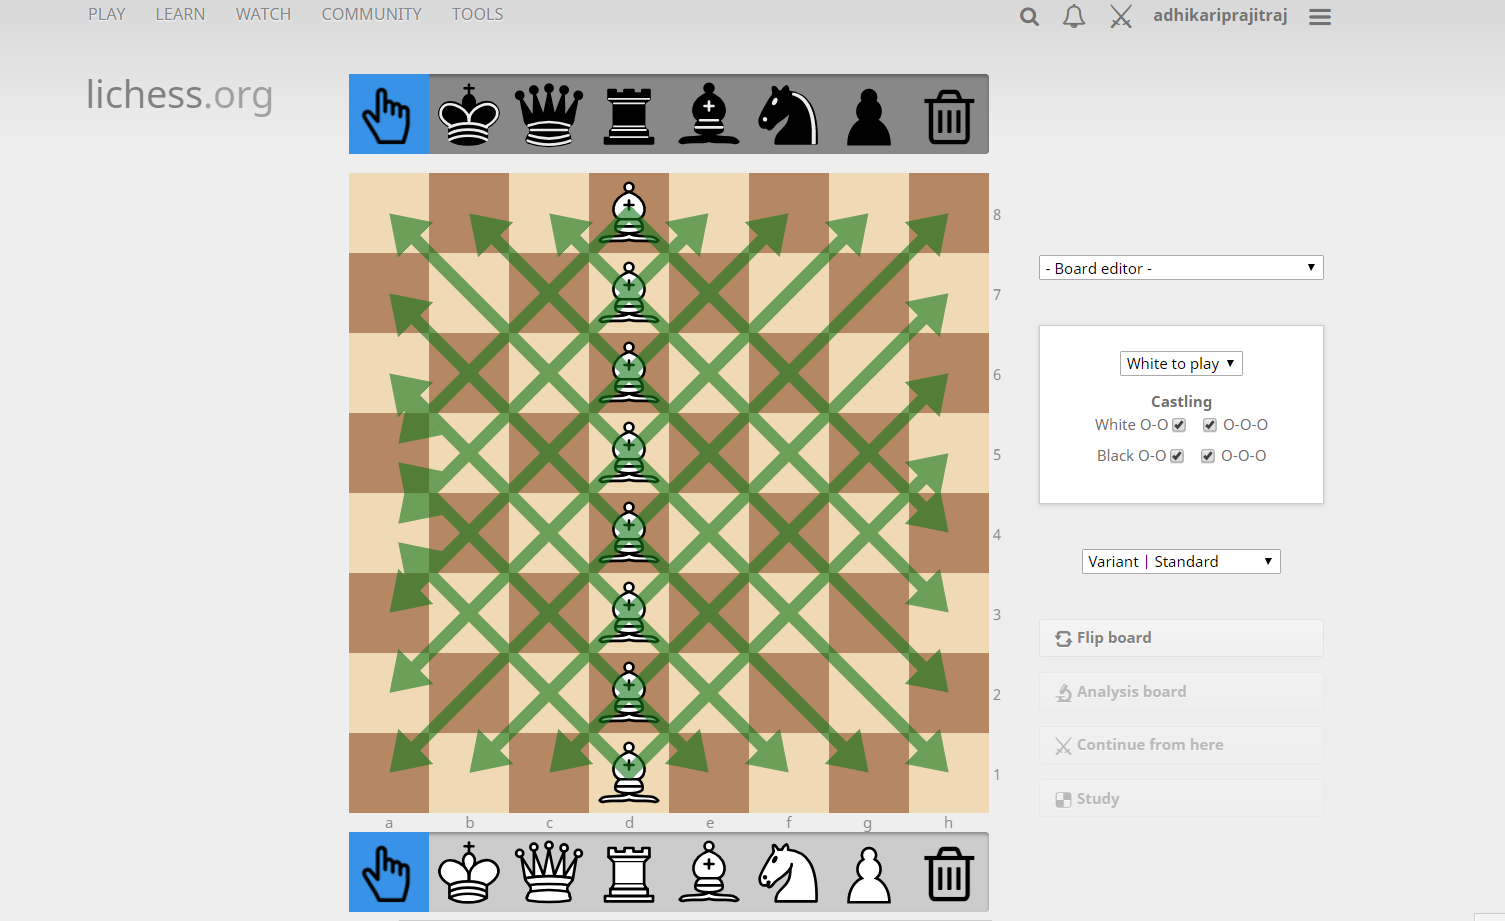
\includegraphics[width=\textwidth]{chess.PNG}







\end{enumerate}




\end{document}